
\documentclass[11pt,a4paper]{article}

% Language and typography
\usepackage[utf8]{inputenc}
\usepackage[T1]{fontenc}
\usepackage[english]{babel}
\usepackage{lmodern}
\usepackage[margin=2.5cm]{geometry}
\usepackage{microtype}

% Black and white color model
\usepackage{xcolor}

\definecolor{primary}{HTML}{000000}
\definecolor{secondary}{HTML}{000000}
\definecolor{codebackground}{HTML}{FFFFFF}
\definecolor{codegreen}{HTML}{000000}

% Figures, tables and diagrams
\usepackage{graphicx}
\usepackage{booktabs}
\usepackage{tikz}
\usetikzlibrary{positioning,arrows.meta}
\usepackage{pgfplots}
\pgfplotsset{compat=1.18}

% Source code formatting
\usepackage{listings}

\lstset{
    language=Python,
    basicstyle=\ttfamily\small,
    keywordstyle=\color{black}\bfseries,
    commentstyle=\color{black}\itshape,
    stringstyle=\color{black},
    backgroundcolor=\color{white},
    numbers=left,
    numberstyle=\tiny\color{black},
    frame=single,
    rulecolor=\color{black},
    breaklines=true,
    showstringspaces=false,
    tabsize=4
}

% Headers and footers
\usepackage{fancyhdr}

\pagestyle{fancy}
\fancyhf{}
\setlength{\headheight}{15pt}

\lhead{\small Cloud Foundations}
\rhead{\small Warehouse Stock Management}
\cfoot{\thepage}

\renewcommand{\headrulewidth}{0.4pt}
\renewcommand{\footrulewidth}{0pt}

% Hyperlinks
\usepackage{hyperref}

\hypersetup{
    hidelinks,
    pageanchor=false
}

\begin{document}

% ================= COVER PAGE =================

\begin{titlepage}
    \centering

    
\includegraphics[width=7cm]{figures/uir-logo.png}\par

    \vspace{0.4cm}

    {\large School of Digital Engineering\par}

    \vspace{2cm}

    \rule{\textwidth}{1.2pt}

    \vspace{0.8cm}

    {\Huge\bfseries CLOUD FOUNDATIONS\par}

    \vspace{0.5cm}

    {\LARGE PROJECT REPORT\par}

    \vspace{1cm}

    {\LARGE Design and Implementation of a
    Cloud-Based Warehouse Stock Management System\par}

    \vspace{0.7cm}

    {\large Microsoft Azure -- Python\par}

    \vspace{0.8cm}

    \rule{\textwidth}{1.2pt}

    \vfill

    \begin{tabular}{ll}
        \textbf{Student 1:} & To be completed \\[0.2cm]
        \textbf{Student 2:} & To be completed \\[0.2cm]
        \textbf{Supervisor:} & To be completed \\[0.2cm]
        \textbf{Academic Year:} & 2026--2027
    \end{tabular}

    \vfill

    {\large Engineering Cycle -- 4th Year}

\end{titlepage}

\hypersetup{pageanchor=true}

% ================= CONTENTS =================

\tableofcontents
\newpage

\listoffigures
\listoftables
\lstlistoflistings
\newpage

% ================= CHAPTERS =================

\section{Introduction}

Managing stock is an important part of the daily
operations of a store. A warehouse may contain a large
number of products from different categories, each with
its own quantity and replenishment needs. Without a
centralized system, keeping track of these products
can become difficult, particularly when stock movements
occur frequently.

The purpose of this project is to develop a web
application that simplifies warehouse stock management
using cloud technologies. The application will allow
users to consult available products and their quantities,
while administrators will be responsible for managing
products and recording incoming and outgoing stock.

Another objective is to reduce the need for manual
inventory monitoring. We plan to introduce an automated
notification system that informs the warehouse manager
when products reach a low stock level or become
unavailable. Statistical features may also be added
to provide a better understanding of stock movements
and replenishment needs.

The project is developed as part of the Cloud Foundations
course at Universit\'e Internationale de Rabat, using
Python as the main programming language and Microsoft
Azure as the cloud platform.

We have chosen to develop the application progressively.
The first stage focuses on establishing a functional
web application and a reliable database. Additional
cloud services will be integrated once this foundation
has been implemented and tested.
\section{Development Environment}

\subsection{Preparation of the Working Environment}

Before starting the implementation, we prepared a local
development environment on Ubuntu. This allowed us to
install and test the necessary tools without consuming
our Azure credits during the initial development phase.

Python was selected as the main programming language,
with Flask as the web framework. Flask provides the
essential features required to build our application
while keeping its structure relatively simple.

We also configured the Azure CLI and Azure Functions
Core Tools to support the later integration and
deployment of cloud services.

\subsection{Development Tools}

Table~\ref{tab:environment} presents the main tools
available in our local development environment.

\begin{table}[htbp]
    \centering
    \caption{Development environment configuration}
    \label{tab:environment}

    \begin{tabular}{lll}
        \toprule
        \textbf{Technology} &
        \textbf{Version} &
        \textbf{Purpose} \\
        \midrule
        Ubuntu & 24.04.5 LTS & Operating system \\
        Python & 3.12.3 & Programming language \\
        Flask & 3.1.3 & Web framework \\
        Werkzeug & 3.1.9 & WSGI utilities \\
        Git & 2.43.0 & Version control \\
        VS Code & 1.146.0 & Development editor \\
        Azure CLI & 2.93.0 & Cloud management \\
        Functions Core Tools & 4.16.1 & Serverless development \\
        LaTeXmk & 4.83 & Report compilation \\
        \bottomrule
    \end{tabular}
\end{table}

\subsection{Python Virtual Environment}

A Python virtual environment was created for the project
to keep its dependencies separate from the packages
installed on the operating system.

After installing Flask, we recorded the installed
dependencies in a \texttt{requirements.txt} file.
This will allow both team members to reproduce the
same Python environment and will also be useful
when deploying the application to Azure.

\subsection{Version Control and Collaboration}

The project is managed using Git, with a remote repository
hosted on GitHub. This provides a common workspace for
the development team and allows us to track modifications
throughout the project.

A \texttt{.gitignore} file was configured to exclude
the virtual environment, sensitive configuration files
and locally generated files that do not need to be
included in the repository.

The application and the LaTeX report are maintained
within the same project directory so that documentation
can progress alongside implementation.
\section{Application Implementation}

\subsection{Initial Flask Application}

We started the implementation by creating a minimal
Flask application. The purpose of this first step was
to verify that our Python environment could run a web
server and return an HTML page to the browser.

The application currently contains a single route
corresponding to the homepage. When this route is
accessed, Flask executes the associated Python function
and renders the HTML template located in the
\texttt{templates} directory.

\begin{lstlisting}[language=Python,
    caption={Initial Flask application},
    label={lst:initial-flask}]
from flask import Flask, render_template

app = Flask(__name__)

@app.route("/")
def home():
    return render_template("index.html")
\end{lstlisting}

\subsection{Client-Server Architecture}

The application follows a client-server architecture.
The browser acts as the client and communicates with
the Flask server through HTTP requests.

Flask receives these requests, executes the appropriate
Python functions and returns a response to the browser.
At this stage, the response is generated from a simple
HTML template. Database operations will be introduced
during the subsequent development phase.

\begin{figure}[htbp]
    \centering

    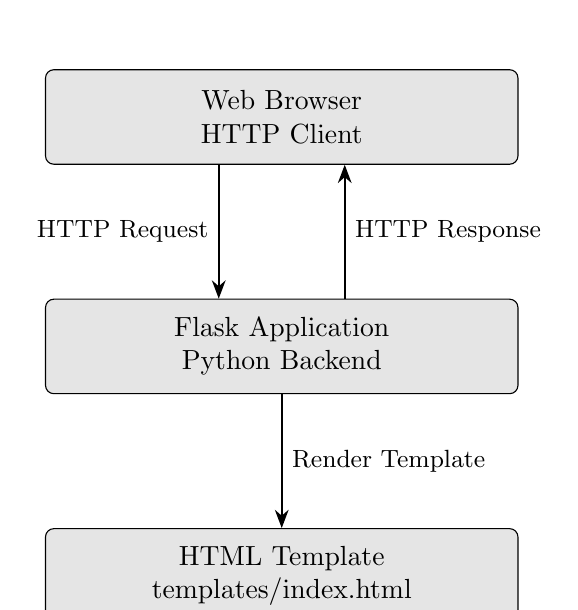
\begin{tikzpicture}[
        node distance=1.7cm,
        component/.style={
            draw=primary,
            rounded corners=3pt,
            fill=primary!10,
            minimum width=6cm,
            minimum height=1.2cm,
            align=center
        },
        arrow/.style={
            -{Stealth},
            thick,
            draw=secondary
        }
    ]

    \node[component] (browser)
        {Web Browser\\HTTP Client};

    \node[component,below=of browser] (flask)
        {Flask Application\\Python Backend};

    \node[component,below=of flask] (template)
        {HTML Template\\templates/index.html};

    \draw[arrow]
        ([xshift=-0.8cm]browser.south)
        -- node[left,font=\small]{HTTP Request}
        ([xshift=-0.8cm]flask.north);

    \draw[arrow]
        ([xshift=0.8cm]flask.north)
        -- node[right,font=\small]{HTTP Response}
        ([xshift=0.8cm]browser.south);

    \draw[arrow]
        (flask.south)
        -- node[right,font=\small]{Render Template}
        (template.north);

    \end{tikzpicture}

    \caption{Initial client-server architecture}
    \label{fig:client-server}
\end{figure}

\subsection{Initial Application Testing}

Once the application was running locally, we used
the curl command-line tool to verify that the server
was responding correctly.

The test was performed by sending an HTTP HEAD request
to the local application address.

\begin{lstlisting}[
    language={},
    numbers=none,
    caption={Local web server verification}
]
curl -I http://127.0.0.1:5000/

HTTP/1.1 200 OK
Server: Werkzeug/3.1.9 Python/3.12.3
Content-Type: text/html; charset=utf-8
Content-Length: 384
Connection: close
\end{lstlisting}

The HTTP 200 response confirms that the requested
page was accessible and that the Flask server was
running correctly.

Although the application does not yet contain any
inventory management features, this first test validates
the basic communication between the browser and the
Python backend. It provides a starting point for the
implementation of the remaining functionalities.

% ==================================================
% Web Application Development
% ==================================================

\subsection{Development of the Web Interface}

Following the initial configuration of the Flask application,
the next step consisted of developing a structured web interface
for the warehouse stock management system.

The interface was designed using HTML and CSS, while Jinja2
was used to connect the frontend to the Flask backend.
A common layout was implemented to maintain consistency
between the different pages of the application.

The main interface contains a navigation sidebar, a header,
and a content area. The homepage provides access to the
inventory module and introduces the administration and
dashboard modules planned for later development.

\subsubsection{Template Inheritance}

Jinja2 template inheritance was introduced to avoid repeating
the same HTML structure across multiple pages. A base template
defines the common elements, while individual templates
contain the content specific to each page.

This approach improves code maintainability and simplifies
future modifications to the application interface.

\begin{figure}[htbp]
    \centering

    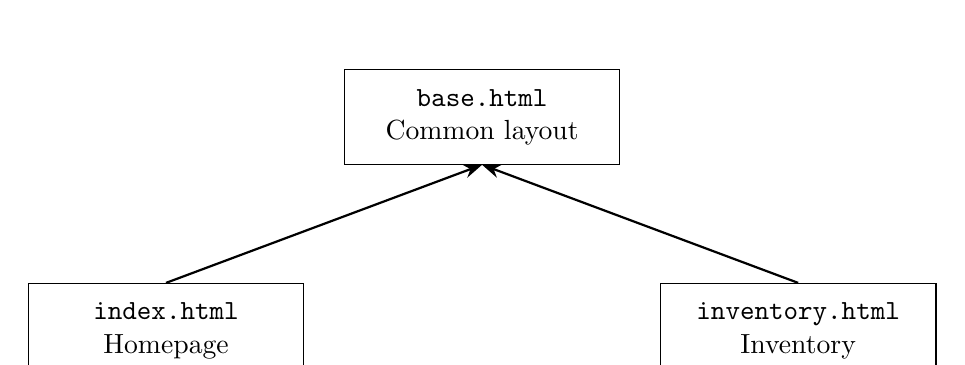
\begin{tikzpicture}[
        component/.style={
            rectangle,
            draw=black,
            fill=white,
            minimum width=3.5cm,
            minimum height=1.2cm,
            align=center
        },
        connection/.style={
            -{Stealth},
            thick
        }
    ]

        \node[component] (base)
            {\texttt{base.html}\\Common layout};

        \node[component, below left=1.5cm and 0.5cm of base]
            (home)
            {\texttt{index.html}\\Homepage};

        \node[component, below right=1.5cm and 0.5cm of base]
            (inventory)
            {\texttt{inventory.html}\\Inventory};

        \draw[connection] (home.north) -- (base.south);
        \draw[connection] (inventory.north) -- (base.south);

    \end{tikzpicture}

    \caption{Jinja2 template inheritance structure}
    \label{fig:template-inheritance}

\end{figure}

% ==================================================
% Product Inventory
% ==================================================

\subsection{Product Inventory Module}

The inventory module allows users to consult the products
available in the warehouse and monitor their stock levels.

During this development phase, six sample products were
defined using a Python list of dictionaries. This temporary
data source allows the functionality of the application
to be tested independently of the cloud database.

Azure Cosmos DB will replace this temporary data source
during a later implementation phase.

\subsubsection{Product Data Model}

Each product contains six attributes describing its
identification, classification, quantity, minimum stock
threshold, and unit price.

\begin{table}[htbp]
    \centering

    \begin{tabular}{lll}
        \toprule

        \textbf{Attribute} &
        \textbf{Data type} &
        \textbf{Description} \\

        \midrule

        id & String & Unique product identifier \\
        name & String & Product name \\
        category & String & Product classification \\
        quantity & Integer & Current stock quantity \\
        min\_stock & Integer & Minimum stock threshold \\
        price & Float & Unit price in MAD \\

        \bottomrule
    \end{tabular}

    \caption{Initial product data model}
    \label{tab:product-model}

\end{table}

\subsubsection{Stock Status Management}

The application determines the status of each product
by comparing its current quantity with its minimum stock
threshold.

Three situations are considered:

\begin{itemize}
    \item \textbf{Available:} the quantity is greater
    than the minimum stock threshold.

    \item \textbf{Low stock:} the quantity is positive
    but does not exceed the minimum stock threshold.

    \item \textbf{Out of stock:} the quantity is zero.
\end{itemize}

These conditions will also serve as the basis for the
automated stock notification mechanisms planned for the
cloud integration phase.

The inventory interface displays the total number of
products, the number of low-stock products, and the number
of out-of-stock products.

% ==================================================
% Search and Filtering
% ==================================================

\subsection{Search and Filtering Mechanism}

To improve product accessibility, a search and filtering
mechanism was implemented within the inventory module.

Users can search for a product by its name or identifier.
They can also filter the catalogue according to product
category and stock status.

The filtering operation is performed on the server side.
The browser sends the selected parameters through an HTTP
GET request. Flask retrieves these parameters, processes
the product data, and returns the matching results through
the Jinja2 template.

Multiple filters can be combined within the same request.
A reset option restores the complete product catalogue.

\subsubsection{Client-Server Communication}

Figure~\ref{fig:filtering-process} illustrates the
communication process between the browser and the Flask
backend during a filtering operation.

\begin{figure}[htbp]
    \centering

    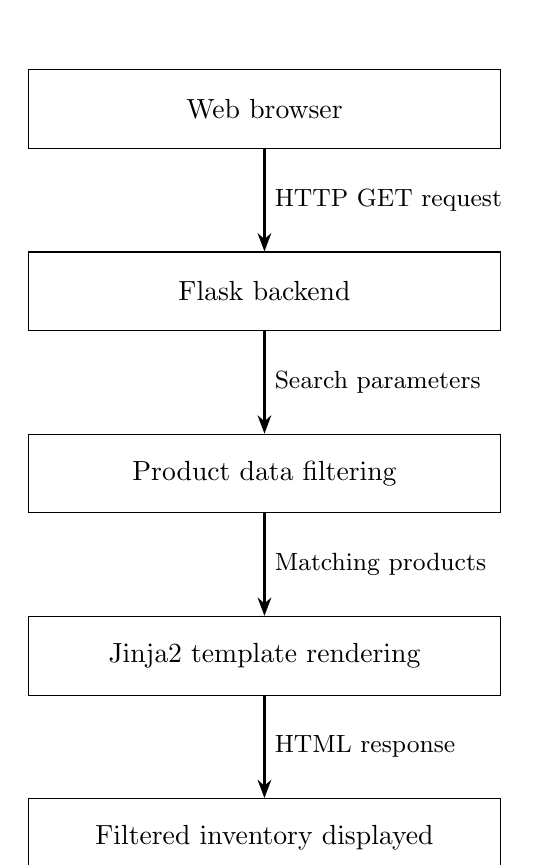
\begin{tikzpicture}[
        node distance=1.3cm,
        component/.style={
            rectangle,
            draw=black,
            fill=white,
            minimum width=6cm,
            minimum height=1cm,
            align=center
        },
        connection/.style={
            -{Stealth},
            thick
        }
    ]

        \node[component] (browser)
            {Web browser};

        \node[component, below=of browser] (flask)
            {Flask backend};

        \node[component, below=of flask] (data)
            {Product data filtering};

        \node[component, below=of data] (jinja)
            {Jinja2 template rendering};

        \node[component, below=of jinja] (result)
            {Filtered inventory displayed};

        \draw[connection]
            (browser) -- node[right, font=\small]
            {HTTP GET request} (flask);

        \draw[connection]
            (flask) -- node[right, font=\small]
            {Search parameters} (data);

        \draw[connection]
            (data) -- node[right, font=\small]
            {Matching products} (jinja);

        \draw[connection]
            (jinja) -- node[right, font=\small]
            {HTML response} (result);

    \end{tikzpicture}

    \caption{Server-side search and filtering process}
    \label{fig:filtering-process}

\end{figure}


% ==================================================
% Application Interface
% ==================================================

\subsection{Application Interface}

The following figures illustrate the results of the
local application development.

\subsubsection{Homepage}

Figure~\ref{fig:homepage} presents the main interface
and its navigation structure.

\begin{figure}[htbp]
    \centering
    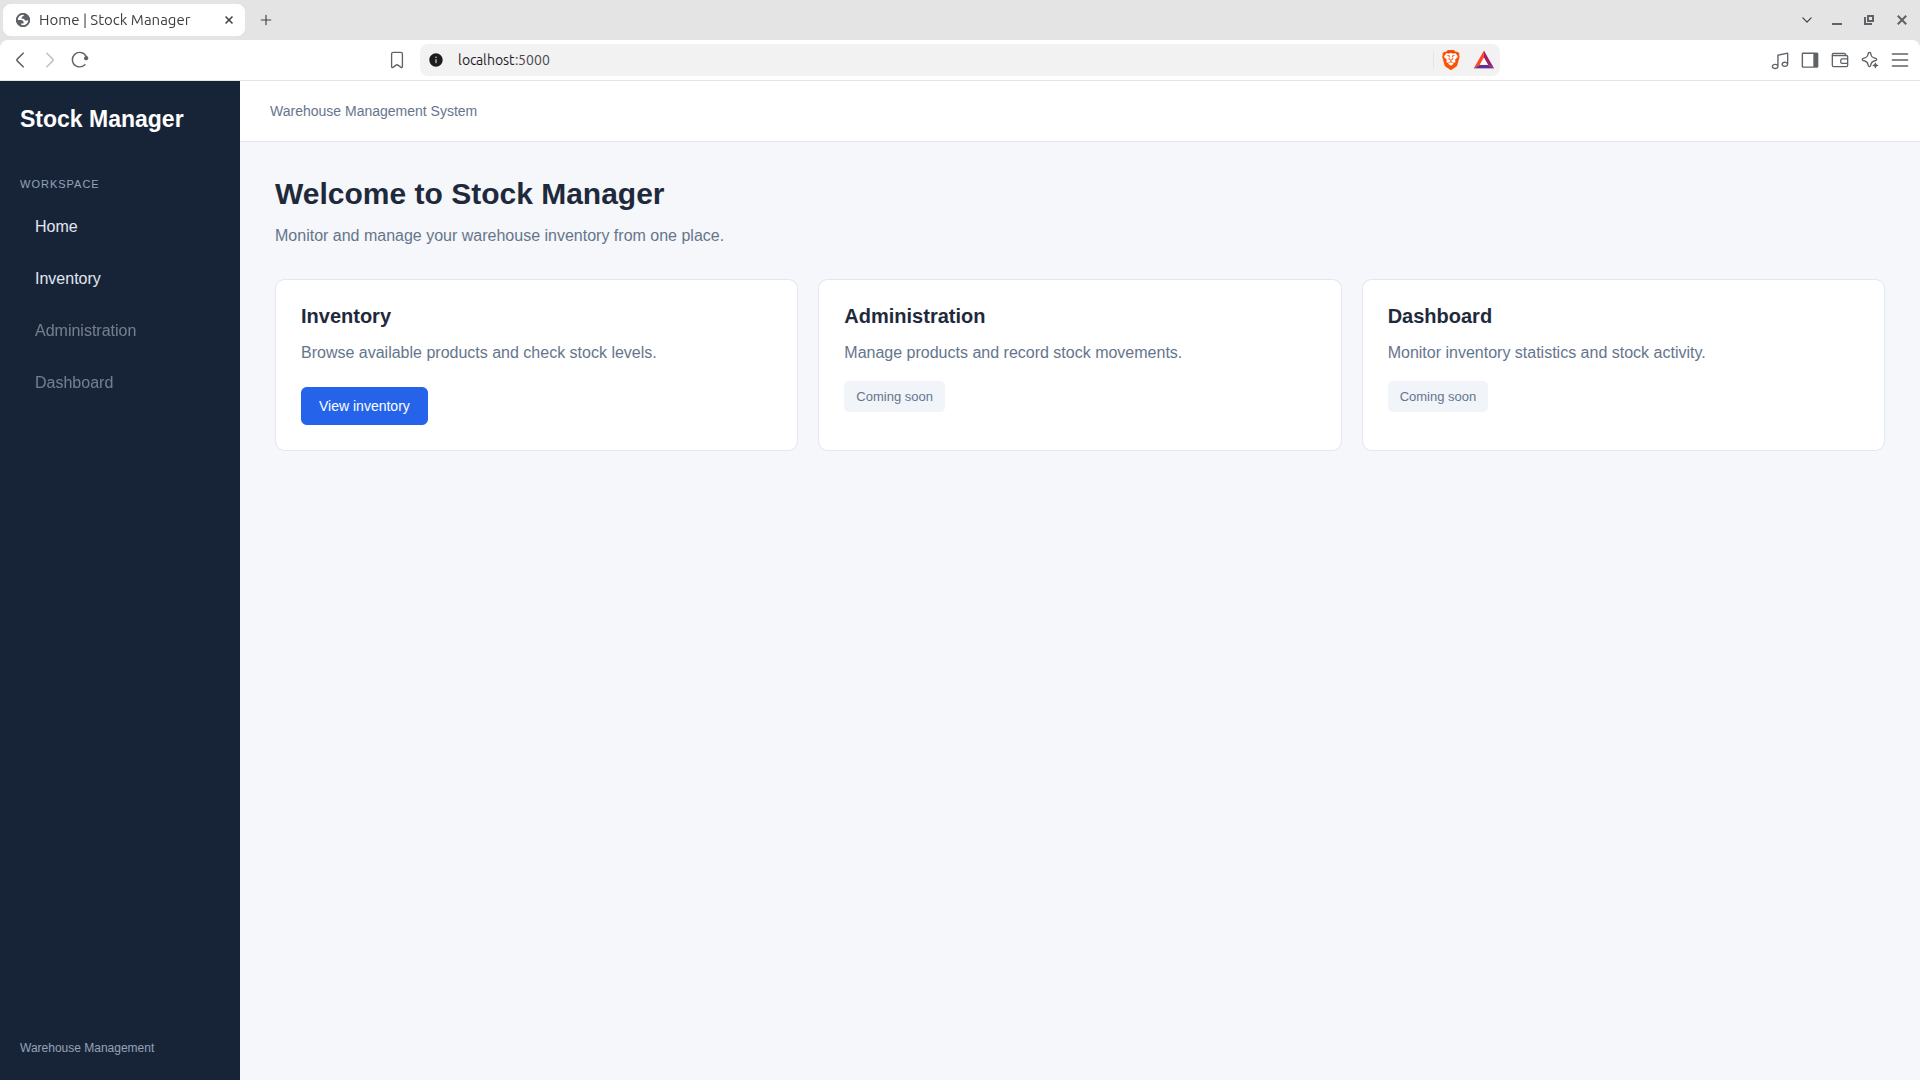
\includegraphics[width=\textwidth]{figures/home.png}
    \caption{Application homepage}
    \label{fig:homepage}
\end{figure}

\subsubsection{Inventory Interface}

Figure~\ref{fig:inventory-interface} shows the product
catalogue and the stock level indicators based on the
six sample products.

\begin{figure}[htbp]
    \centering
    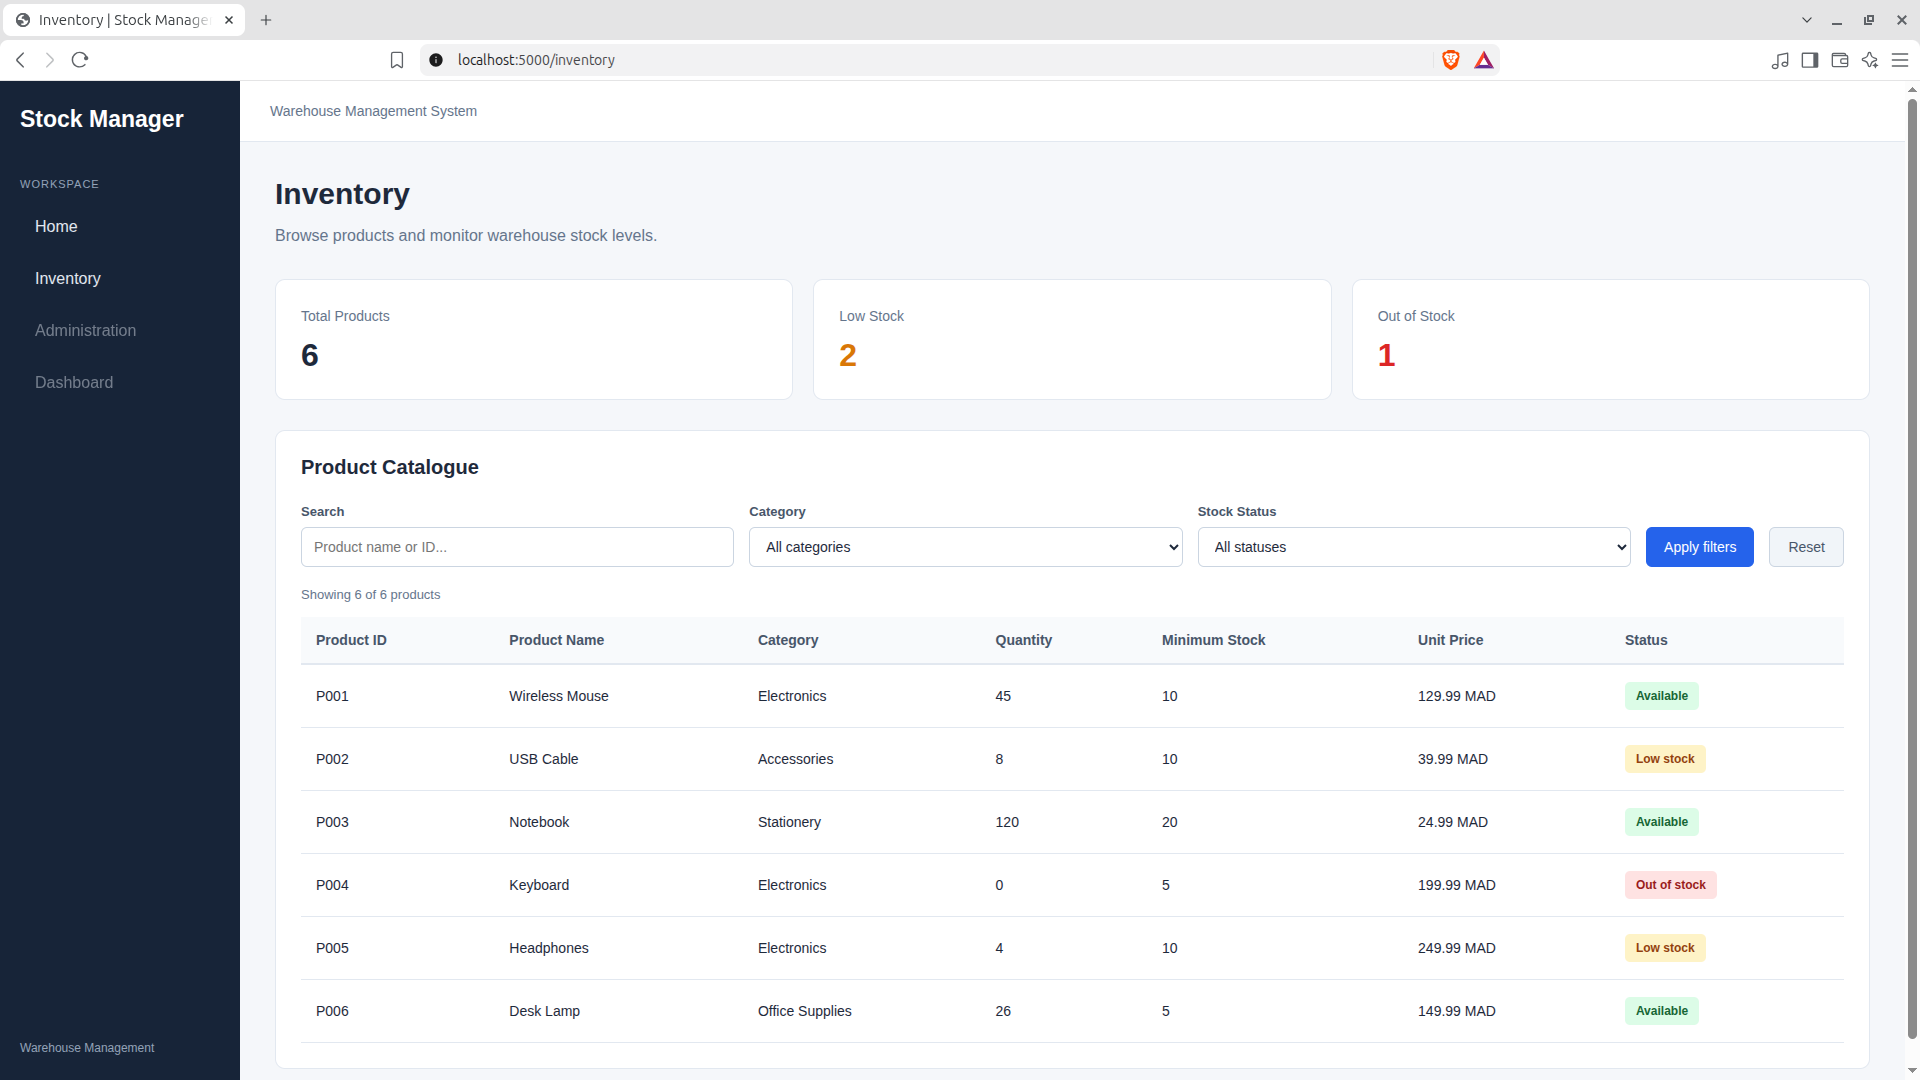
\includegraphics[width=\textwidth]{figures/inventory.png}
    \caption{Product inventory interface}
    \label{fig:inventory-interface}
\end{figure}

\subsubsection{Search and Filtering Results}

The combination of the Electronics category and the
Low stock status returns a single product, as shown
in Figure~\ref{fig:filtered-inventory}.

\begin{figure}[htbp]
    \centering
    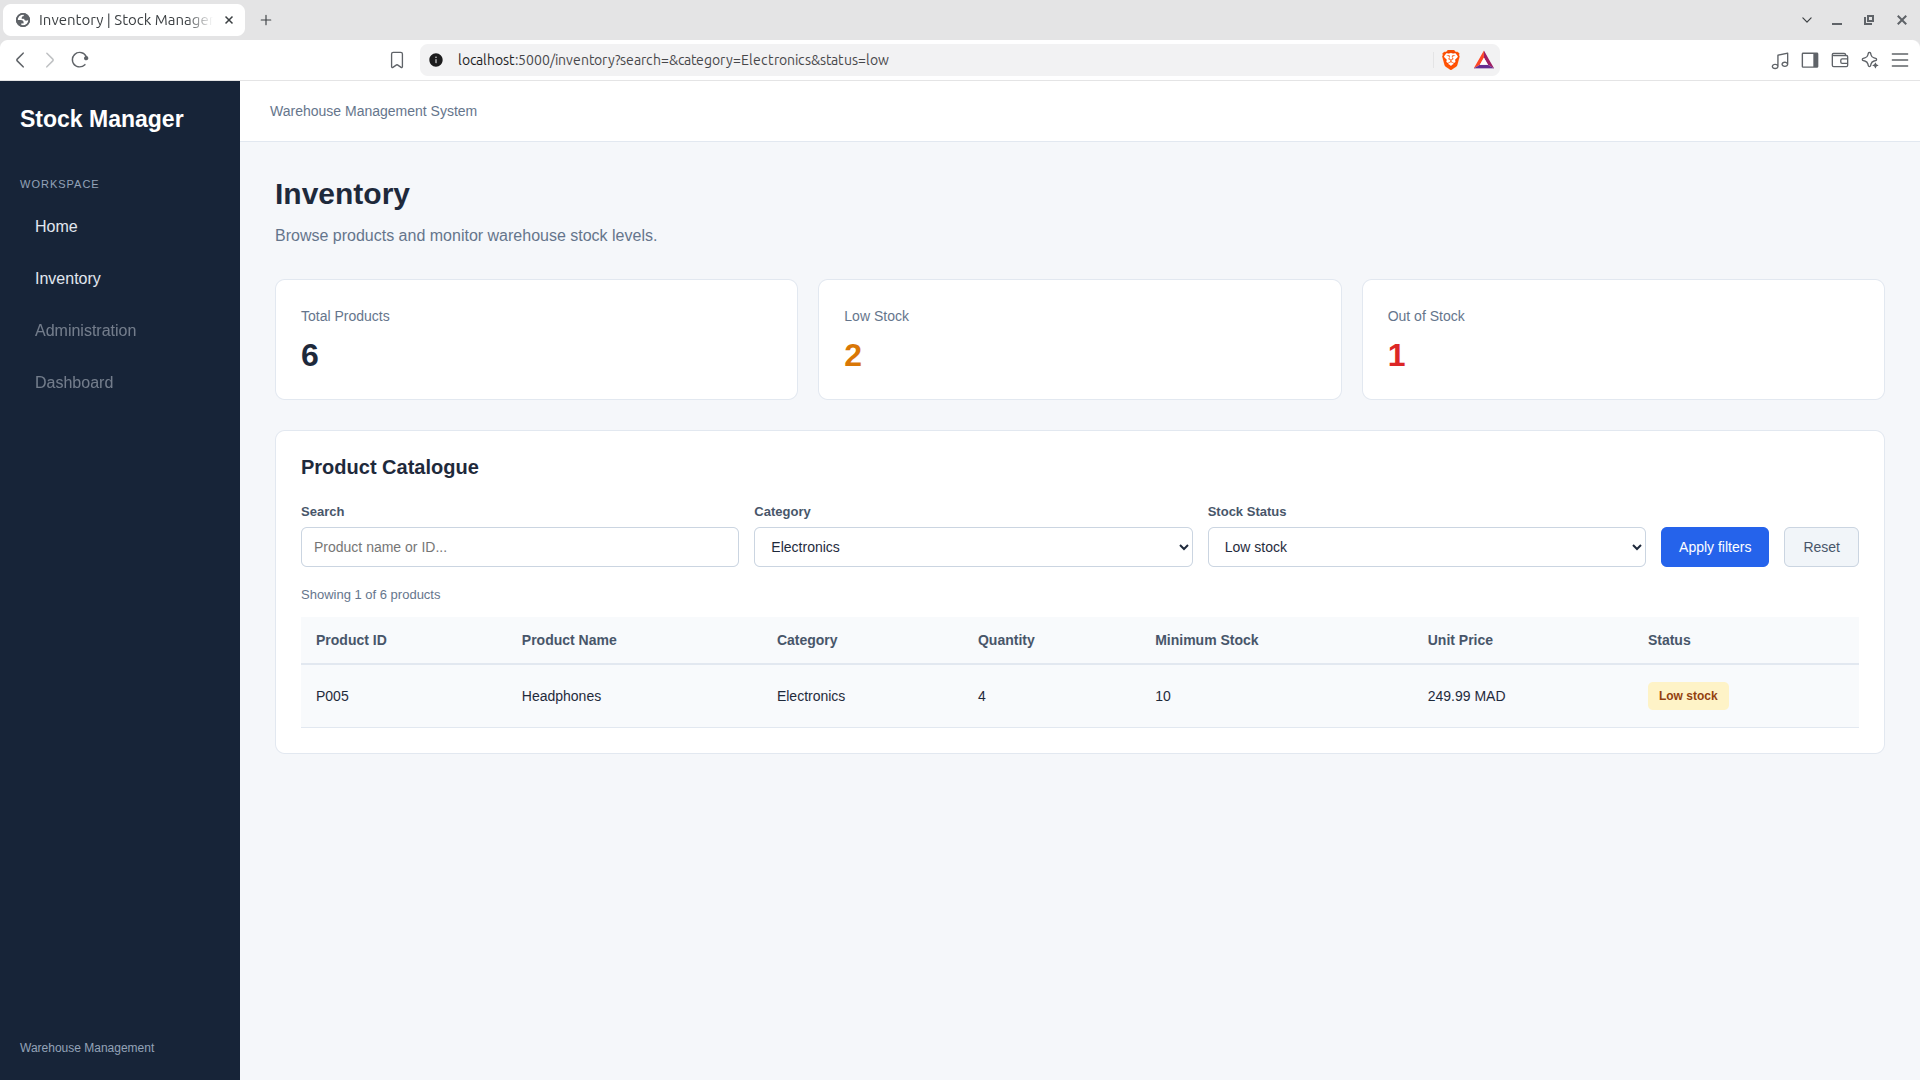
\includegraphics[width=\textwidth]{figures/inventory-filter.png}
    \caption{Inventory results after applying combined filters}
    \label{fig:filtered-inventory}
\end{figure}

% ==================================================
% Functional Testing
% ==================================================

\subsection{Functional Testing}

Nine functional tests were performed locally to
validate the search and filtering mechanism.

\begin{table}[htbp]
    \centering
    \small

    \begin{tabular}{cllc}
        \toprule

        \textbf{No.} &
        \textbf{Test scenario} &
        \textbf{Expected result} &
        \textbf{Result} \\

        \midrule

        1 & Search: mouse & 1 product & Passed \\
        2 & Search: P003 & 1 product & Passed \\
        3 & Electronics category & 3 products & Passed \\
        4 & Available status & 3 products & Passed \\
        5 & Low stock status & 2 products & Passed \\
        6 & Out of stock status & 1 product & Passed \\
        7 & Electronics and low stock & 1 product & Passed \\
        8 & Unknown product search & No results & Passed \\
        9 & Reset filters & 6 products & Passed \\

        \bottomrule
    \end{tabular}

    \caption{Inventory module functional testing results}
    \label{tab:inventory-tests}
\end{table}

All nine tests passed, validating the inventory
module against the defined functional requirements.

The application currently operates locally using
temporary product data. Cloud integration will be
addressed in the next development phases.


\end{document}
